\documentclass{beamer}
%\documentclass[notes=only]{beamer}

\usepackage[utf8]{inputenc}
\usepackage{listings}
\usepackage{ulem}
\usepackage{hyperref}
\usepackage{amsmath}

\lstdefinestyle{customcbig}{
  belowcaptionskip=1\baselineskip,
  breaklines=true,
%  frame=L,
  xleftmargin=\parindent,
  language=C,
  showstringspaces=false,
  basicstyle=\small\ttfamily,
  keywordstyle=\bfseries\color{green!40!black},
  commentstyle=\itshape\color{purple!40!black},
  identifierstyle=\color{blue},
  stringstyle=\color{orange},
}

\lstdefinestyle{customc}{
  belowcaptionskip=1\baselineskip,
  breaklines=true,
%  frame=L,
  xleftmargin=\parindent,
  language=C,
  showstringspaces=false,
  basicstyle=\scriptsize\ttfamily,
  keywordstyle=\bfseries\color{green!40!black},
  commentstyle=\itshape\color{purple!40!black},
  identifierstyle=\color{blue},
  stringstyle=\color{orange},
}

\lstdefinestyle{customctiny}{
  belowcaptionskip=1\baselineskip,
  breaklines=true,
%  frame=L,
  xleftmargin=\parindent,
  language=C,
  showstringspaces=false,
  basicstyle=\tiny\ttfamily,
  keywordstyle=\bfseries\color{green!40!black},
  commentstyle=\itshape\color{purple!40!black},
  identifierstyle=\color{blue},
  stringstyle=\color{orange},
}
 
\usetheme{Dresden}

\title[SOFTENG 370 Tutorial 7 (2019)] %optional
{Exam Revision}
  
\author{Edward Zhang}
 
% \institute[UoA] % (optional)
% {
%   Department of ECSE\\
%   The University of Auckland
% }
 
\date[October 2019] % (optional)
{SOFTENG 370 T7}

\begin{document}
\frame{\titlepage}
\begin{frame}
  \frametitle{Exam Info}
  Your exam will be short answer, not MCQ. That means the exam from 2012 - 2017 aren't very useful. 2018 had a different lecturer for the first $\frac{1}{2}$ so it's not super helpful either.\\
\end{frame}
\section{Adapted MCQs}
\begin{frame}
  \frametitle{Instructions which query the running state of a processor (i.e. kernel or user mode) make virtualization difficult. Why?}
  \pause
  Consider trap and emulate virtualization, where we expect privileged instructions from the guest to throw exceptions that the VMM can trap.
  \pause
  \begin{block}{Answer}
    An instruction running in the kernel of a guest operating system would report that it was running in user mode.
  \end{block}
\end{frame}
\begin{frame}
  \frametitle{In order to allow safe multiprogramming what hardware advances needed to be made?}
  \pause
  Key word: Safe. How can we keep tasks isolated from each other (recall we need two things for this, one alone won't work), and how do we allow for effective time sharing?
  \pause
  \begin{block}{Answer}
    Hardware memory protection, interrupt processing, privileged instructions.
  \end{block}
\end{frame}
\begin{frame}
  \frametitle{Which of the following statements about files is FALSE?}
  \begin{itemize}
    \item All Unix files are stored on secondary storage.
    \item With sparse files it is possible to have the size of a file larger than the device the file is stored on.
    \item Executable files have different structures specific to their particular operating systems.
    \item Moving a file does not necessarily mean that all of the data needs to be copied then the original file deleted.
  \end{itemize}
  \pause
  \begin{block}{Answer}
    All Unix files are stored on secondary storage. Counterexample: \texttt{tmpfs}
  \end{block}
\end{frame}
\begin{frame}
  \frametitle{Which of the following statements about NFS is TRUE?}
  \begin{itemize}
    \item NFS only works in a homogeneous environment with all clients and servers running the same operating system.
    \item Servers in NFS are dedicated to acting as file servers and cannot be used for general operations.
    \item NFS mounts remote directories in a similar way to the method Unix mounts drives in the directory tree.
    \item Remote file directories in NFS can only be mounted when a machine is booted.
  \end{itemize}
  \pause
  \begin{block}{Answer}
    NFS mounts remote directories in a similar way to the method Unix mounts drives in the directory tree. Recall that NFS maintains a mapping of directories to remote servers that they're mounted on.
  \end{block}
\end{frame}
\begin{frame}
  \frametitle{Which of the following is NOT usually considered a requirement in a language used for operating system implementation?}
  \begin{itemize}
    \item It is easy to produce fast and efficient code with the language.
    \item The language allows access to memory locations.
    \item The language is compiled.
    \item The language is dynamic and weakly typed
  \end{itemize}
  \pause
  \begin{block}{Answer}
    The language is dynamic and weakly typed. Counterexample: We don't usually write OSes in Javascript lol
  \end{block}
\end{frame}
\begin{frame}
  \frametitle{Which of the following best describes the Confused Deputy problem?}
  \begin{itemize}
    \item A program with privileges is tricked into giving those privileges to another program.
    \item A program with privileges is tricked into misusing its authority.
    \item A program with privileges gets so many requests that it loses track of which request came from which source.
    \item A program with privileges mistakenly prevents access to a resource which should be available. 
  \end{itemize}
  \pause
  \begin{block}{Answer}
    A program with privileges is tricked into misusing its authority. i.e. You ask the deputy (say \texttt{passwd}) to do something for you that it shouldn't (change someone else's password) and it obliges.
  \end{block}
\end{frame}
\begin{frame}
  \frametitle{Order these file block allocation techniques from most efficient to least efficient for random access to file information.}
  “Efficient” for this task relates to the number of different block reads necessary to access the file information
  \begin{itemize}
    \item Single-level Indexed allocation
    \item Contiguous allocation
    \item Multi-level Indexed allocation
    \item Linked Allocation
  \end{itemize}
  \pause
  \begin{block}{Answer}
    Contiguous allocation (trivial), single-level indexed allocation (access only one index block), multi-level indexed allocation (access multiple index block), linked allocation (linked-list like).
  \end{block}
\end{frame}
\begin{frame}
  \frametitle{Describe locality of reference and why it is important?}
  Consider in the context of virtual memory and also filesystems, especially network ones.
  \pause
  \begin{block}{Answer}
    Many memory or file accesses in a small period of time are close together. This is important for the efficiency of virtual memory (loading in memory from swap), read-ahead in file data and in distributed file systems.
  \end{block}
\end{frame}
\begin{frame}
  \frametitle{Which of the following statements best describes what is being depicted in the figure?}
  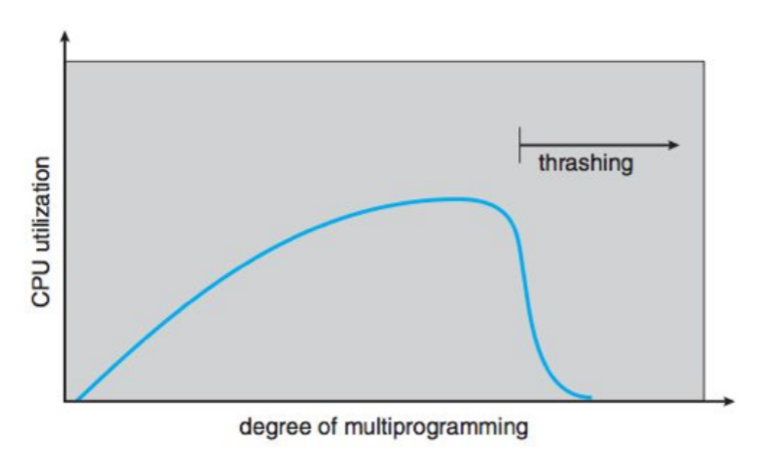
\includegraphics[width=\textwidth,height=0.8\textheight,keepaspectratio]{images/thrashing.png}
\end{frame}
\begin{frame}
  \frametitle{Cont.}
  \begin{itemize}
    \item Running too many processes can cause thrashing in the virtual memory system which means that very little work can get done by any process.
    \item Increasing the amount of multiprogramming will increase the CPU utilization until the file system can no longer deal with the read/write requests and the hard drives crash.
    \item Increasing CPU utilization allows the number of processes to increase until a limit is reached and most of the processes finish.
    \item When thrashing begins the amount of free CPU time goes up dramatically this means that more processes can now be scheduled.
    \item All of the above.
  \end{itemize}
\end{frame}
\begin{frame}
  \frametitle{Answer}
  \begin{itemize}
    \item<alert@+|+-> Running too many processes can cause thrashing in the virtual memory system which means that very little work can get done by any process.
    \item Increasing the amount of multiprogramming will increase the CPU utilization until the file system can no longer deal with the read/write requests and the hard drives crash.
    \item Increasing CPU utilization allows the number of processes to increase until a limit is reached and most of the processes finish.
    \item When thrashing begins the amount of free CPU time goes up dramatically this means that more processes can now be scheduled.
    \item All of the above.
  \end{itemize}
\end{frame}
\end{document}